%!TEX encoding = MacOSRoman
%!TEX TS-program = xelatex
%!BIB TS-program = bibtex

% --------------------- Start of Document Preamble -----------------------

\documentclass[12pt, oneside]{report} % report is suitable for the long document such as Ph.D thesis with chapters
\usepackage[a4paper, left=1in, right=1in, top=1in, bottom=1in]{geometry} 
\usepackage{fontspec}
\setmainfont{Times New Roman}
\usepackage{pdflscape}
\usepackage{apacite}
%\usepackage[round]{natbib}  % the bibliography
\usepackage{sectsty}
\chapterfont{\centering}
\usepackage{enumitem} % enumerate package
\linespread{2}
\usepackage{amsmath,amssymb,amstext} % Lots of math symbols and environments
\usepackage{graphicx} % For including graphics N.B. pdftex graphics driver 

%----- Adjust the style ----
\renewcommand{\chaptername}{CHAPTER}
\renewcommand{\thechapter}{\Roman{chapter}}
% ---------------------- End of Document Preamble ------------------------

%======================================================================
%   L O G I C A L    D O C U M E N T -- the content of your thesis
%======================================================================
\begin{document}

% For a large document, it is a good idea to divide your thesis
% into several files, each one containing one chapter.
% To illustrate this idea, the "front pages" (i.e., title page,
% declaration, borrowers' page, abstract, acknowledgements,
% dedication, table of contents, list of tables, list of figures,
% included into the document by the following statement.
%----------------------------------------------------------------------
% FRONT MATERIAL
%----------------------------------------------------------------------
% T I T L E   P A G E
% -------------------
% Last updated May 24, 2011, by Stephen Carr, IST-Client Services
% The title page is counted as page `i' but we need to suppress the
% page number.  We also don't want any headers or footers.
\pagestyle{empty}
\pagenumbering{roman}

% The contents of the title page are specified in the "titlepage"
% environment.
\begin{titlepage}
        \begin{center}
        \vspace*{0.5cm}

        \normalsize
        {\bf NETWORK ANALYSIS OF RICE HEALTH SUREVEY DATA FOR CHARACTERIZATION OF YIELD REDUCING FACTORS AND YIELD LIMITING FACTORS OF TROPICAL RICE ECOSYSTEM IN SOUTH AND SOUTHEAST ASIA}

        \vspace*{4.0cm}

        \normalsize
        \bf{SITH JAISONG} \\

        \vspace*{4.0cm}

        \normalsize
        THESIS OUTLINE SUBMITTED TO THE FACULTY OF GRADUATE SCHOOL\\
        UNIVERSITY OF THE PHILIPPINES LOS BA\~NOS\\ 
 IN FULFILLMENT OF THE \\
        REQUIREMENT FOR THE \\ 
        DEGREE OF \\
        \vspace*{2.0cm}
        PH.D OF SCIENCE \\
        (Plant Pathology) \\

        \vspace*{1.0cm}
%        \copyright\ Pat Neugraad 2007 \\
        May 2015
        \end{center}
\end{titlepage}

% The rest of the front pages should contain no headers and be numbered using Roman numerals starting with `ii'
\pagestyle{plain}
\setcounter{page}{2}

\cleardoublepage % Ends the current page and causes all figures and tables that have so far appeared in the input to be printed.
% In a two-sided printing style, it also makes the next page a right-hand (odd-numbered) page, producing a blank page if necessary.
 
%------------Setting the bibliography style --------------



%------------End of the bibliography style ----------------

% D E C L A R A T I O N   P A G E
% -------------------------------
  % The following is the sample Delaration Page as provided by the GSO
  % December 13th, 2006.  It is designed for an electronic thesis.
%  \noindent
%I hereby declare that I am the sole author of this thesis. This is a true copy of the thesis, including any required final revisions, as accepted by my examiners.

%  \bigskip
  
%  \noindent
%I understand that my thesis may be made electronically available to the public.

%\cleardoublepage
%\newpage

% A B S T R A C T
% ---------------

%\begin{center}\textbf{Abstract}\end{center}

% You're not characterizing different environments. They're all tropical, irrigated, lowland rice
%Characterising rice agroecosytems requires knowledge and information of qualitative and quantitative information. One way of gathering data the data necessary for this is through the conduct of surveys. Given the nature of the data, it is not a simple task to analyse and examine in order to derive information and knowledge. One method in particular, network analysis, has been used to explore the observed relationships between the individual elements in a given system. This study is the first known attempt to apply network analysis to the analysis of in-field and household survey data on rice yield limiting and reducing factors. The data will be analyzed and visualized using the proposed network model. I propose to construct a network model using survey data collected from 2009 to 2011 in several sites (Chekempek, West Java, Indonesia; Mekong River Delta, Vietnam; Tamil Nadu, India; and Suphaburi, Thailand) and test the model with data collected from 2012 to 2015 in several cropping seasons and sites (Chekempek, West Java, Indonesia; Red River Delta, Vietnam; Tamil Nadu and Odisha, India; Suphaburi, Thailand). The anticipated results from this research will be helpful for plant health authorities worldwide, in order to design specific strategies for rice pest and disease management and to limit the impacts of these yield reducing factors. 


%\cleardoublepage
%\newpage

% A C K N O W L E D G E M E N T S
% -------------------------------

%\begin{center}\textbf{Acknowledgements}\end{center}

%I would like to thank all the little people who made this possible.
%\cleardoublepage
%\newpage

% D E D I C A T I O N
% -------------------

%\begin{center}\textbf{Dedication}\end{center}

%\cleardoublepage
%\newpage

% T A B L E   O F   C O N T E N T S
% ---------------------------------
\renewcommand\contentsname{TABLE OF CONTENTS}
\tableofcontents
\cleardoublepage
%\phantomsection
%\newpage

% L I S T   O F   T A B L E S
% ---------------------------
%\addcontentsline{toc}{chapter}{List of Tables}
%\listoftables
%\cleardoublepage
%\phantomsection		% allows hyperref to link to the correct page
%\newpage

% L I S T   O F   F I G U R E S
% -----------------------------
\addcontentsline{toc}{chapter}{LIST OF FIGURES}
\listoffigures
\cleardoublepage
%\phantomsection		% allows hyperref to link to the correct page
%\newpage

% L I S T   O F   S Y M B O L S
% -----------------------------
% To include a Nomenclature section
% \addcontentsline{toc}{chapter}{\textbf{Nomenclature}}
% \renewcommand{\nomname}{Nomenclature}
% \printglossary
% \cleardoublepage
% \phantomsection % allows hyperref to link to the correct page
% \newpage

% Change page numbering back to Arabic numerals
\pagenumbering{arabic}
 

%----------------------------------------------------------------------
% MAIN BODY
%----------------------------------------------------------------------
% Because this is a short document, and to reduce the number of files
% needed for this template, the chapters are not separate
% documents as suggested above, but you get the idea. If they were
% separate documents, they would each start with the \chapter command, i.e, 
% do not contain \documentclass or \begin{document} and \end{document} commands.

%======================================================================
% INTRODUCTION
\chapter{INTRODUCTION}
%======================================================================
%=========================
%INTRODUCTION
%=========================
%\section*{Introduction}
\addcontentsline{toc}{chapter}{Introduction}
% 1. Why are you talking in past tense in your opening sentence? I already commented about being consistent in your verb tenses.
% 2. Sentence 2 should be part of sentence 1.
% 3. "at irrigated areas" is awkward. It should be "in irrigated areas"
% 4. No "," after "approximately".
% 5. Your punctuation in the entire para is a shambles.
% 6. This para is out of place. It needs to be in your M&M for the section.

Pests and diseases to global rice production are significant yield reducing factors. \shortciteA{OERKE:2006ct} estimated that rice pests potentially caused losses around 37 percent of global rice production. Additionally, future rice production will need to grow by 2.4 percent per year in order to meet the demands of a growing population \shortcite{Ray:2013by}. Addressing these yield-reducing factors is essential for food security not only in rice consuming societies, but also for other societies societies globally.

% 1. The sentence starting with "A survey" doesn't need a ","
% 2. Did Serge just imply or did he state that management strategies should be developed according to patterns?
% 3. Last sentence is a bit unclear. Revise.

Nowadays, developing the strategies of pest and disease management takes into account sustainability, production efficiency, and environmental protection \cite{Mew:2004kh}. To achieve this, interactions between pests and human activities must be studied. A survey may provide the necessary data, and adequate methods for analyzing survey data can produce preliminary information on their behaviors including major interactions \shortcite{savary1995use}. \shortciteA{Savary:2000vr} concluded that the observed injury profiles (i.e., the combination of disease and pest injury that may occur in a given farmer’s field) were strongly dependent on production situation. It was implied that pest management strategies should be developed according to the patterns of cropping practices, and production situations. However, interactions among pests, cropping practices, and environments are difficult to elucidate. Moreover, most previous analytical techniques can not be used to reveal their changes across locations or time, which they are important to design the strategies of pest management. 

Network analysis provides a promising tool for revealing the interactions among entities within a complex system. It has been applied for many branches of science (e.g., social science, computer science, biology). A network model is an abstract model composed of a set of nodes or vertices and a set of edges, links or ties connected to the nodes. Nodes usually represent entities and the edges represent their relations. For example, an ecological network of a food web presents nodes as species \shortcite{krause2003compartments} and edges as ecological relationships, or consider a social network of students in the school present where nodes are students and edges are friendships \shortcite{moody2001race}.

%-----------------------------
\section*{OBJECTIVES}
\addcontentsline{toc}{chapter}{Objectives}
%----------------------------

% 1. Confused. I thought that this was basically a proposal for your disseration. Why are your goals written in past-tense? Are they not present or future, you've not completed the work yet, unless I'm unaware.
% 2. You don't need commas before every "and", I've seen this at least twice in this section alone
% 3. Third objective, different levels of yield gains? I'm unclear on what you mean here. Yield gains have a very specific meaning, how are you studying them?

My overall objective was to develop network approaches, and apply them to analyze crop health survey data. My first objective for this research was to develop the network model based on crop health survey data and characterize relationships among components of injuries and cropping practices. My second objective was to compare the differential relationships of network models under different seasons or locations. The third objective was to compare differential patterns of their relationships at different levels of yield gains.

% 1. Again, verb tense. Is this work that you've already done? If so, why are you submitting this to the graduate school?
% 2. Grammar in first sentence and second sentence

Once network models based on crop health survey data were constructed, they can be helpful for plant health authorities, and the people who related to crop protection especially for rice. The models support them to design specific strategies for rice pest and disease management and to limit the impacts of these yield reducing factors.  

% eos


\chapter{REVIEW OF LITERATURE}
%====================================
% introduction of literature review
%===================
\section*{Introduction}
\addcontentsline{toc}{section}{Introduction}
%==================

The applications of network analysis have increased exponentially over the past two decades in various disciplines. Even though documented applications of network analysis in plant pathology are still relatively sparse, network applications in the social sciences, systems biology and ecology have been increasingly found. Here I review the empirical works that exist and argue that network analysis is a promising approach for exploring questions in the context of plant pathology.

% 1. You don't discuss all four sections here. What's in the fourth section?
%Sith There are only three sections, not four
% 2. Your sentence starting with "Network analysis provides..." is out of place. The rest of this para after that point belongs somewhere else IN the lit review, not in a description of what you'll tell reviewing.

%This chapter contains three sections to thoroughly review of network analysis and its applications. In the first sections, I introduce a brief overview of the concepts and methods of network analysis, and I then discuss the unique values of network analysis that are not found in other approaches. In the third section I focus on the application of network analysis to current applications of plant pathology research, in particular, plant disease epidemiology and molecular plant pathology, for which network analysis has been broadly applied, and increasingly documented. Network analysis provides fruitful tools for visualizing, analyzing and understanding complex relationships in the studies of plant disease. For instance, network models of genes or proteins pertaining plant defense mechanisms and network models revealing spatial distribution of plant disease through trade networks were already reviewed by \citet{windram2014network} and \citet{Shaw:2014cka}, respectively.
%The last section presented analytical techniques and strategies to apply network analysis for studying pest management. It introduces three strategies of network applications, which are developed and applied in the studies of systems biology and ecology, and concludes the brief discussions of potential applications to the studies of crop heath management that have yet been undertaken.

\section*{Network Analysis}
%==========================
\addcontentsline{toc}{section}{Network analysis}
% Good
\subsection*{Introduction to network analysis}
% Your opening paragraph here is repetitive. You've already established this point before. Move these references into the body and start with your next paragraph.
Network analysis is used for determining relationships between elements of interest. It offers toolkits for visualizing data in a network model and measuring its properties, and network thinkings \citep{PROULX:2005hx}. It has been widely used by various branches of science, such as social science, ecology, biology, computer science, and many others to study the interactions between elements, e.g., the relationships of students in school \citep{moody2001race}, species in food webs \citep{krause2003compartments}, interactions of genes or proteins in cells \citep{guimera2005functional}, or the connections of computer in the network \citep{pastor2001epidemic, newman2006modularity}.

% Good
\citet{newman2003structure} loosely categorized four types of networks based on different complex data. The first category is social network, representing sets or groups of people forming some patterns of contacts or interactions between them such as the patterns of friendship or business relationships. Analyzing the structure of whole social entities gives us the perspectives from a social network, which enables us to explain the patterns observed. \citet{moody2001race} analyzed the social behaviors in high school students using social network approaches. \citep{Kasari2011social} applied network analysis to compare the social relationships and friendships between children with and without autism spectrum disorder (ADS). The second type of network is an information network or knowledge network. The classic example of this network is the network of citations between academic papers \citep{newman2003structure}. The articles cited other papers, which have related topics. They formed a citation network that has vertices as articles and direct links as citations. The citation network visualizes the structure and the movement of the information. The third category, technological network, is object connected network, or man-made network which represents a physical connection between objects. This network is mostly applied for illustrating physical structures and systems such as the electrical power grid, the connections of rivers, transport systems, etc. The fourth category of network is a biological network. It represents the biological systems such as genes to genes, genes to protein, protein to protein interactions, which enable biologists understand the connections and interactions between individual constituents including genes, proteins, and metabolites at the level of the cell, tissue and organ to ultimately describe the entire organism system. Biologists use biological networks in various branches of biology at different levels (from a single molecule to an entire organism). For example, \citet{yang2014gene, barabasi2004network} studied in the patterns of gene expression in different conditions and different types of cells (normal cells and cancer cells) in order to characterize the genes that change and do not change following the particular conditions; \citet{freilich2010large} applied a molecular ecological network analysis to study the communities of soil microorganisms. Networks revealed the complex relationships between microbial species in soils and their communities. Moreover, network analysis enables ecologists to understand ecological properties and predict the ecological roles of species in a soil ecosystem. Although the application of each type of network approach varies, all four categories of networks share a common empirical focus on relational structure and a similar set of mathematical analysis. 

%% Add more to this para. Also, don't recite the same papers that you've already cited. This is a good place to move Windram and Shaw from above (they're already here so remove them above...).
Network analysis can be a powerful tool to study plant disease. \citet{Lefebvre:2011fo, Jeger:2007tn} applied network models and concepts to study disease spreads in regional networks of plant nurseries and garden centers of \textit{Phytophthora ramorum}, the oomycete causing Sudden Oak Death in the West Coast of the USA and leaf blight and dieback in many ornamental shrubs both in America and Europe. The result could be applied to design measures to control plant disease epidemic from movement of infected material among plant nurseries. \citet{Shaw:2014cka} recently reviewed critically about network analysis to plant disease management (\textit{i.e.}, to design ways to reduce the flow of disease in traded plants, to find the best sites to monitor as warning sites for annually reinvading diseases, to understand the fundamentals of how plant pathogen spreads in different structures of simulated trade network models). \citet{windram2014network} reviewed the applications of network analysis in molecular plant pathology. Network models were applied to reveal plant defense mechanism during plant-pathogen interactions.

\subsection*{Concepts, principles, and methods of network analysis}

A network represents relationships between of elements of interest, which are defined by links (edges) among nodes (vertices). Nodes can be units of interests or studies, and links represent interactions between nodes. Network analysis aims to identify the patterns of associations among nodes, not only features or attributes of particular nodes.

Network analysis follows three principles. Nodes and their behaviors are mutually dependent, not autonomous; links between nodes can be channels for transmission of both material (\textit{e.g.}, money, disease) and non-material (\textit{e.g.}, information, knowledge, relationship, interaction) and; persistent pattern of association among nodes create structure that can define, enable, or restrict the behavior of a node.

Network models have two different organizational structures depending on goals of the representation and analysis \citep{borgatti2013analyzing}. Flow models, commonly named directed graphs, view the network as a system of pathways along which something move such as transportation networks (\textit{e.g.}, of highways, railways and airlines) or communication networks. Since flow networks show the directions of movement between nodes, thus these networks are interesting to study their behaviors. Analysis of flow networks can identify which nodes are more active or which ones are more important connectors. \citet{Jeger:2007tn, Shaw:2014cka} applied such network models to study plant disease spread. Architectural models, or indirected graphs, are mainly used to determine the structure of the network, seeking to discern whether specific structures lead to similar outcomes or whether nodes in similar network positions behave in similar ways. Ecological applications related to the ecology and spatial structure of ``community'' tend to be organized and analyzed as architectural models. For example, \citet{Faust:2012dk} studied networks of soil microbial interactions. Network models can describe how microbial populations change over time, which will require the use of dynamic models of microbial communities. Beyond these basic principles, network analysis enables the calculation of structural properties of nodes, groups, or the entire network.

\textit{Measuring network properties}

%% LaTex quotes... yes it should be ``sith''
A network is made up of nodes and links from relational data. It is constructed from an adjacency matrix, which is obtained from analysis using metric algebra techniques. The row and column headings for an adjacency matrix are identical, listing the names of the components involved in the network. In the simplest case, the cells of the matrix are coded with ``1'' if a link exists between the node or ``0'' if no edge exists. However, a link can be valued. Value indicates a characteristic of the relationship that the research has quantified. The values may be binary, such as whether two friends recognize each other, or variable strength (\textit{e.g.}, the number of mutual friends between two friends). A network link need not imply positive or cooperative interaction; they can also be a negative or competitive interaction between two individuals. 

The distribution of links in a network suggests two important structural characteristics: centrality (importance) of nodes in the network and division of the network into subgroups. Variants of centrality in a network include degree, closeness, and betweenness. Degree centrality of a node is the sum of the value of the links between that node and every other node in the network. This measure tells us how well-connected a particular node is to the other nodes. Closeness centrality is calculated using the length of the path between a node and every other node. This measure could estimate the time required for information or resources to propagate to a given node in a network. Betweenness centrality corresponds to the number of paths in the network that pass through a particular node, and therefore measures the dependence of a network on a particular node for maintaining connectedness \citep{Toubiana:2013cv}. \citet{Deng:2012do, newman2003structure, Toubiana:2013cv} are recommended references for descriptions of the theory and uses, as well as the formal calculation of these measures.


%==========================
\section*{The unique values of network analysis}
\addcontentsline{toc}{section}{The unique values of network analysis}
%==========================

There are four key points that will help to understand network analysis 1) how it differs from traditional approaches of scientific research; 2) how it relates to those traditional approaches; 3) how networks are constructed, manipulated and measured; and 4) what value network analysis offers beyond traditional approaches.

The first point of network analysis is that there are two types of data represented in the network graphs; technical and rational data. The first is data characterizing the actors or variables being studied referring to attributes. Attributes describe characteristics of individual actors or variables, for example their race, income or physical location, and are the primary variables considered in traditional approaches. The second type of data is relational data, that is, data about the relationships between individual nodes. For example, \citet{Lazega} represented the network model of cooperation among lawyers in three law firms, through the exchange of various type of resources among them. This model consisted of over 70 lawyers in three different offices in three different cities. Rational data reflected to resources exchange and additional attribute information were included type of practice, genders, and seniority of each lawyers.

Relationships are also referred to as edges (links) in network analysis. Edges cannot be attributed to any single actor. Rather, edges only exist between nodes. This leads to the second point about network analysis that it requires a different conceptual approach. Because edges only exist between nodes, it is useful to think of edges existing in a separate dimension from nodes, who are connected in physical space. This dimension is sometimes referred to as relational space. To visualize the difference, think of someone far away with whom you correspond regularly, say using a phone, email, or Facebook. Even though the two of you are not physically close, you have a strong relationship. The two of you are distant in physical space but close in relational space. This notion of relational space is in part what means when he refers to the space of flows as something distinct from the space of places \citep{Castells}.

The third point that distinguishes network analysis from other approaches is it involves different methods of analysis. Because traditional research methods consider variable attributes in a wide variety of statistical analyses such as measures of center (\textit{e.g.}, mean, median, etc.) and dispersion (e.g., standard deviation, range, etc.), these methods are sometimes referred to as variable analysis, whereas, network analysis models relational data and to measure various characteristics of network structure. For example, for lawyers data \citep{Lazega}, it is natural to ask to what extend two lawyers that both work with third lawyer are likely to with each other as well. This notion corresponds to the social network concept of transitivity and can be captured numerically through an enumeration of proportion of vertex triples that form triangles, so-called cluster coefficient. 

The idea that network structure may be correlated with variable attributes and behaviors is the fourth point to consider in comparing network analysis to other approaches. In network analysis, the arrangement of the network in relational space is basically correlated with the behavior and attributes of those variables. For example, in the network created by \citet{Lazega} lawyers of the same firm may share similar attributes such as office location or department, and lawyers in similar roles within that network may share similar behaviors. Basically, conventional approaches measure various attributes of variable (nodes in a network) and attempts to discern something about the relationships between actors (edges in a network) based on those attributes. When the network structure is simple and the differences in node attributes are clear, the conventional analytic approach is sufficient. However when relationships are complex or node attributes are more nuanced, clear answers using conventional analysis may prove elusive. As a result, network analysis offers a tool to help researchers visualize the large network and disentangle some of the relational complexities within the network, just as cluster analysis and multivariate analysis for help research disentangle the complex data.

\section*{Networks and Plant Pathology}
\addcontentsline{toc}{section}{Networks and Plant Pathology}

%% You've cited Jeger, Lefebvre and Windram 2X each already. That's 2X more than necessary to establish that plant pathologists use this method. The more specific examples are probably fine here though.
Recently, a broad expansion of applications of network analysis has occurred across many disciplines. It has been evaluated as a promising tool to study a complex system. Plant pathologists have applied network analysis for their research. \citet{Lefebvre:2011fo, Jeger:2007tn, windram2014network} supported that network analysis can be fruitful models in many applications relevant to plant pathology because of its generality and flexibility. For example, the network of main fresh cut flowers movements among European countries was determined the likelihood of introduction of new pathogens and other organisms associated with plants \citep{eagling2007australian}, and plant-pathogen interaction network models were applied to present plant defense mechanisms \citep{dietz2010hubs}. 

The development of network analysis challenges conventional approaches to uncover rational complexities of plant pathology studies. Two fields of research relevant to plant pathology presented particularly strong growth and proved that network analysis has significant potential to augment traditional analysis methods. The first is plant disease epidemiology, which investigates questions related to plant disease spread. The second is plant molecular biology, which investigates questions related to biological networks.

\subsubsection*{Using Network analysis to understand plant disease spread}
\addcontentsline{toc}{subsection}{Using Network analysis to understand plant disease spread}

Network analysis challenges conventional approaches of studies in plant disease epidemiology, especially underling the spatiotemporal flow of plants and their pathogens \citep{Moslonka2010}. When plant pathological studies were restricted to a single geographical location, there was a limit to thinking about the connections or relationships between plants or fields in different locations. However, network analysis can enlarge the view of studies and can consider whether or not plant pathogens are moving from one field to others in the regions of interest. For example, networks of plant disease spread in trade networks presented the flows of plant disease from infected units (infected plants or epidemic areas) to susceptible units (susceptible plants or areas).

\textit{\textbf{Network models of epidemic development}}
 
 % this is the 4th? time you've cited Lefebvre, what's new?
The idea of plant epidemics is that the probability of infection embedded in the connection or the contact patterns between susceptible/infected plants, and it forms as the networks. \citet{pautasso2010number} showed a network model of epidemic development (susceptible-infected-susceptible model) in a directed network. In the network model, vertices were represented plant, and their attributes were presented the infectious status (healthy or infected). The epidemic is started at a single node, then nodes with a connection from the starting infected node will be infected at the next time step with a certain probability of transmission. In turn, already infected nodes will be infected at the next time step depending on their infection status and on a certain probability of persistence. The probability of infection transmission is the same for all connections between infected nodes and susceptible nodes over times. Similarly, the probability of infection persistence is the same for infected nodes in a certain network replicate. For each network structure, the two probabilities of persistence and transmission define an epidemic threshold, which is independent of the starting node of the epidemic. This epidemiological model does not result in either susceptible or infected nodes, as nodes will have a infection status along a continuum. Key quantities for epidemiological dynamics in networks were reviewed in \citet{Lefebvre:2011fo}.

\textit{\textbf{Analysis of plant trade network}}

% You already said this about Jeger, what's new?
\textit{Phytophthora ramorum} epidemic networks in the horticultural trade are an example of the application of network models in the study of plant disease spread \citep{harwood2009epidemiological, Moslonka2010}. Simulations of spread of \textit{P. ramorum} in different network structures (random, small--world and scale--free network) were found that epidemic threshold, the boundary between a no epidemic an epidemic outcome, is significantly lower for scale-free network, a network is dominated by a small number of nodes with many connections, compared to local, random and small-world network structure. Modeling suggested that was possible to control an epidemic by changing the structure of network, without having to decrease the probability of infection persistence at a nursery site and/or of transmission between sites. Simulation showed that correlation coefficient between link in and out nodes increased with connectivity level for all the structures investigated and underlined the importance of targeted control towards node with more connections than others. 

%% Fix. "The scenario where there are major nodes which both receive plant material from many production sites and supply many retail sites is the most problematic control of this control s target towards such hubs."
%% No idea what this means. Clarify. " Simulations showed that the number of equilibrium. This correlation increase with connectivity level for all the structures investigated and underlines the importance of targeted control towards node with more connections than others \shortcite{Moslonka2010}."

Regardless of the network structure and connectivity level, epidemic threshold is negatively correlated to the correlation coefficient between link in and out nodes, \citep{Moslonka2008}. In presence of high-connected nodes, the most effective way to control disease spread is to move from two-way to a one-way network. That is move from network where overall there is positive correlation among links-in and -out to one where the correlation are negative. In practice this would mean that a nursery network would be dominated by major node, which receives plant materials from many production sites but supply relatively few retail sites, or by major nodes which received plant materials from a few production sites but supply many retail sites. However, the scenario where there are major nodes which both receive plant material from many production sites and supply many retail sites is the most problematic control. The better way to control should target towards the cluster (group of nodes), not only to high-connected nodes. 

The last point, the modeling of disease spread in small-size directed networks showed that increasing the proportion of wholesalers (\textit{i.e.}, traders without a preponderance of incoming or outgoing links) tends to decrease the epidemic threshold in local, random, and small-world network. The opposite result is obtained for the proportions of produces and retails. Scale free networks appear instead to be tolerant to changes in these hierarchical categories as the epidemic threshold in this case is governed by the presence of hub rather than by the features of the majority of nodes in the network \citep{Moslonka2010}.

\textit{\textbf{Network models to design strategies of plant disease management}}

Due to globalization, plant trades among countries are increasing and convenient. They potentially caused risks to plant health when they were not under good control. To control the risks of plant disease epidemic through plant trade, network models were applied to present the flows of trade network of plants and plant products across the world and within countries and to develop strategies of plant disease management \citep{pautasso2015network}. Networks could be found hubs or highly connected nodes, which represented locations or countries where imported and exported plants or plant parts. Hubs or highly connected nodes were targets for control disease flows in the scenarios that network presented because they were considered to the likelihood of pathogens actually infecting along particular links. Strategies for disease management should be designed by focusing on links to and from hubs, nodes which have high degree of connectivity, so that it increase efficiency to control plant pathogen spreads. The strategies may aim to remove them from the network \citep{Jeger:2007tn, Lefebvre:2011fo}. Alternatively, strategies may pay attention on them in order to prevent disease spreads. \citet{Shaw:2014cka} suggested placing quarantine efforts on hubs or on connections between major hubs.

Additionally, \citet{pautasso2008epidemiological} showed the good examples, which are co-occurrence networks of the \textit{Phytophthora ramorum} infected plant genera different environments. The networks may be helpful in identifying host taxa playing an important role in spreading a certain disease in the seminatural environment, in crop plants, and plants in the trade. Combining genetic network analysis and data on trace forward and trace back on movement of plants nursery trade supported to identified confidentially \textit{P. ramorum} migration. From this approach, it was clear that the pathogen was introduced originally from nurseries, which \textit{P. ramorum} populations in nurseries are genetically ancestral to all Californian forest populations.

\subsubsection*{Using Network analysis to understand molecular plant pathology}
\addcontentsline{toc}{subsection}{Using Network analysis to understand molecular plant pathology}

% this subsubsection seems awfully short? I would think more network analysis has been used in bioinformatics than ecoinformatics for plant pathology, yet this section is shorter?
For understanding mechanisms of plant-pathogen interactions, network analysis offers tools to visualize interactions of biological components including genes, proteins, and metabolites, which are related to plant-pathogen interactions. Network concepts enable us to characterize interplay of those components following the properties of network structure. Analyzing structural properties of networks may provide useful clues about the biological functions of individual genes, genes complexes, proteins, protein complexes, pathways they participate in.

\textit{\textbf{Presenting biological data with network model}}

Networks are used in different contexts as ways to represent relationships between entities, such as interactions between genes, proteins or metabolites. \citet{wu2007gene} gave the example of a network model built from gene-for-gene relationships between rice and various avirulence genes of the pathogen \textit{Xanthomonas oryzae} pv. \textit{oryzae} causing bacterial leaf blight of rice. Nodes were represented isogenic lines of rice and weighted edges reflected the number of shared genes with high resistance (with respect to avirulence genes) in the two isogenic lines of rice. For a plant breeder, this graph can help in identifying particularly promising genes for developing a disease resistant variety.


\textit{\textbf{Network analysis to study biological systems}}

%% First sentence is still unclear
Network analyses have been applied to visual the myriad information and analyzes the complex relationships. To better understand the collective impact of genes on complex traits and determine what governs their organization, biologists are most likely to apply gene co-expression networks \citep{usadel2009co}. Co-expression networks most commonly use the Pearson's correlation coefficient to establish linear pairwise correlations between gene pairs in an adjacency matrix. Another associative metric that can be used is the Spearman correlation coefficient, which captures nonlinear correlations between genes to be uncovered \citep{usadel2009co, horvath2011weighted}. Once a co-expression network has been generated, identifying modules by clustering can help extract biological meaning from the network. Uncharacterized genes within such a module can be candidates for participating in the same process. Similarly, genes directly connected to (or co-expressed with) known central regulators of a developmental process are candidates within this co-functional framework.

% write the summary this part need to review some of variable and analysis the concepts 
% Last sentence is unclear. Revise.
% defense mechanisms in the pathogen or the host?
\citet{Zheng2013} used co-expression network inference to investigate plant imunity system of citrus in response to\textit{Candidatus} Liberibacter asiaticus. Gene coexpression networks based on Pearson's correlation coefficients using four transcriptomic data sets studies of citrus infected by \textit{Candidatus} Liberibacter asiaticus bacterium were constructed. The result showed high degree of preservation of gene co-expression patterns across the networks based on different datasets. The network structures revealed hub genes, which have high connectivity. Highly connected nodes (genes) were closely related to Arabidopsis SYP71 encoding a plant syntaxin which functions as a plasma membrane- associated protein transporter. Furthermore, in the study of \citet{mukhtar2011independently}, plant-pathogen interaction networks revealed the interactions of novel \textit{Arabidopsis} protein-pathogen effectors, provided evidences that pathogen effectors target a limited number of host immune proteins, and demonstrated that effectors from very distantly related pathogens interact with the same host proteins. 

The main use of co-expression networks with large collections of static expression data is gene discovery. However, many biologists have attempted to construct differential networks to measure differences in connectivity patterns from datasets with different conditions or targeted experiments \citep{Toubiana:2013cv}. \citet{Lu:2013hga} constructed networks of soil fungal communities. The fungal networks represented two different conditions; yield-invigorating and yield-debilitating soils under prolonged potato monoculture were compared. The authors discussed in differential network concepts that in healthy network three-eighths of fungal groups and soil organic matters were strongly correlated, and in diseases network two of four groups strongly correlated with soil electrical conductivity (EC) and ammonium nitrogen. Differential network analysis showed that average degrees of nodes belonging to \textit{Sordariales} and \textit{Hypocreales} in healthy network substantially were different in disease network. This indicated that they are key species of ecological communities.

\section*{A Variety of Network Construction Methods}
\addcontentsline{toc}{section}{A Variety of Network Construction Methods}

Until this section, I gave the general information of network analysis with network concepts, network modeling and inference. Ultimately, most of the systems studied from a network--based perspective are dynamic in nature. This underscore the importance of developing tools to understand the interplay between network structures and dynamical processes. I reviewed three network-based analysis: single network, differential network and dynamic network analysis. These techniques from network science have yielded many biological insights\citep{Idekerdiffne}. 

\textbf{\textit{Single Network Analysis}}

Single-network analysis will be used for analyzing a network based on a single data set. It aims to model patterns of relationships between entities to a network, thereby determining its topological properties such as node degree, degree distribution, average path length, clustering coefficient, modularity index \citep{newman2006modularity} to describe the patterns in the network model. These structural properties offer the potential to explore relationships within complex data sets and identify key factors or clusters.

Correlation based networks are widely used for studying biological networks based on pair--wise correlations between variables. Their edges are obtained using correlation-based measures removing spurious relationships. Correlation based measures include linear based correlation (Pearson's correlation, partial correlation) and rank based correlation (Spearman's correlation, Kendall's correlation). Removal of spurious relationships is particularly important when one attempts to establish causal relationships between entities \citep{Toubiana:2013cv}. A correlation based network allows one to define modules (clusters), intramodular hubs, and network nodes with regard to module membership, to study the relationships between modules, and to compare the network topology of different network. 

\textbf{\textit{Differential Network Analysis}}

Networks can respond differently under various environments or with external signals. They can be simplified by focusing on key components and capture only the essential components differently responding between environments in which they play a key role in the modeled response \citep{Peer:2011jd}. Networks are examined by adding or deleting some variables. This allows predicting interactions or components that change following the changed structure of networks. 

Differential network analysis is applied to identify and describe differences between two networks under different conditions. Differential networks from different data sets with different conditions might display different interactions from the single network based on the whole data set, which are disregarded the conditions. The strongest interactions in differential networks are not necessarily those that are strong in the single network. Conversely, they may be weak or absent in single network. Compared between differential networks under different environment conditions, the differential interactions can be implied that they are a result of response to environmental conditions. Moreover, it can be implied that environments influence on the interaction between pairs of nodes contributing to the differential interactions. 

The objective of differential network analysis is to identify the different interactions, that may reveal when condition has changed. For example, the differential network analysis of gene co--expression networks to understand the differences between human and chimpanzee brain was focused on how expression patterns of genes were different in human and chimpanzee brains. These networks are contrasted to find a) non-preserved modules (group of genes with sharing similar expression profiles and presumably similar functions), b) differentially occurred genes, and c) differentially connected genes. The result showed that 

\textbf{\textit{Dynamic Network}}

Biological systems are highly dynamic. They must continuously respond to external signals or the internal state of the system. The responses can be altered slowly or quickly over time \citep{Peer:2011jd}. Thus, realistically the corresponding biological network models must evolve as well. It seems clear that dynamic networks enable us to see and understand the systems and how their dynamic effects change over time. Some understandings previously have been obtained from studies of dynamics of large networks, for example, gene expression or metabolic fluxes network \citep{Idekerdiffnet}.

The main goal of dynamic network analysis moves away from single network analysis, which characterizes absolute properties of the system. It aims to concentrate on a specific dynamic response. Rather than answer what the key factors in the system, it answers what parts of the system are most affected by perturbation. Most commonly, dynamic networks are applied when the edges among a set of vertices or the sets of vertices itself are changing as a function of time. For example, 


\section*{Summary}
\addcontentsline{toc}{section}{Summary}

This literature review presented a brief introduction of network analysis and concise concepts and methods. Briefly, a network is usually represented by sets of nodes (or vertices) connected by edges (or links) in various ways. Networks can be categorized to four types, social network, information, technology network, and biological network. Even though four types of networks are described and applied in different context, they share a common empirical focus on relational structure and a similar set of mathematical analyses. Network models are cable of presenting unique values, which traditional approaches cannot present. Network analysis was discussed as applied to two broad areas of study of plant diseases. It firstly was applied to study plant disease epidemics. For example, networks of textit{Phytophthora ramorum} spread through plant nurseries trade. The results enabled us to understand the directions and processes of disease spread. Additionally, they could predict the movement of disease flows, and improve the implementation of plant disease policy. Secondly, molecular plant pathology showed two applications of network applications. The first use is to apply networks to model large and complex biological datasets. Another use is the consideration network structure to understand biological system. Emergent properties of network structure influences may be identified, measured and analyzed to yield better explanations of the experiments being observed. While numbers of documented plant pathological studies using network analysis are sparse, the literature presented in this review showed a clear and compelling case for plant pathologists to expand the understanding of and use network concepts and methods. 
Biological networks are context-specific and dynamic in nature. Under different conditions, the topology of the network changes. Network approaches (differential network, dynamic network analysis) are successful to yield insight on biological system under different conditions or dynamic processes. Network analysis concepts and methods augment existing approaches and provide tools for exploring complex relationships, which have been widely acknowledged as influential but difficult to measure using traditional methods. 

% eos

%======================================================================
% Materials and Methods
\chapter{MATERIALS AND METHODS}
%======================================================================
%=========================
% Materials and Methods
%=========================

% Your not including yield in your analysis? Seems to be a big reason for this work. Why is it not included?
This research will use data collected from surveys of irrigated lowland rice growing areas in South and South East Asia to examine relationships between the injuries caused by pests and diseases, cropping practices (\textit{e.g.}, rice variety grown, crop establishment method, fertilizer and chemicals applied). Their relationships will be constructed and analyzed through network analysis. I will develop and apply suitable methods of network analysis to characterize the associations of injuries and cropping practices. The resulting network of associations of injuries and cropping practices will thus provide a starting point for further investigations of their relationships (\textit{i.e.}, characterization of relationships of cropping practices and injury profiles related to yields, comparison of networks under different production environments or examination of networks at different levels of yield gains). 

In the following, I present three distinct network analysis approaches: single-network analysis, differential network analysis, and dynamic network analysis. These three approaches will answer different questions. I will apply single-network analysis to the data from all fields surveyed for identifying patterns of interactions between injuries and cropping practices and key components (\textit{e.g.}, most connected variables). Second, differential network analysis will aim to uncover similarities and differences of networks constructed from the different data sets (\textit{e.g.}, dry season versus wet season). Dynamic network analysis, the third type, will be applied to study how networks changed under at least two different aspects of an evolving complex system. Here, I will focus on dynamic networks by dividing farms into different levels of yield attained. 

\subsection*{Crop health survey data}
\addcontentsline{toc}{subsection}{Crop health survey data}

% how many farmers' fields were surveyed?
Crop health survey data were collected through surveys of farmers' fields (approximately 800) from 2010 to 2015 for both wet and dry seasons in different production environments across South and South East Asia representing irrigated lowland rice growing areas West Java, Indonesia; Mekong River Delta and Red River Delta, Vietnam; Tamil Nadu and Odisha, India; and Suphanburi, Thailand. The survey protocol described in the IRRI publication, ``A SURVEY PORTFOLIO TO CHARACTERIZE YIELD-REDUCING FACTORS IN RICE'', \citep{Savarysurvey2009} was used for data collection. The variables collected included environmental attributes, patterns of cropping practices, crop growth measurement and crop management status assessments, measurements of levels of injuries caused by pests, and direct measurements of actual yields from crop cuts. The data collected can be classified into three groups: cropping practices, injuries, and actual yield measurements.

Cropping practice data included information on the type of rice variety (traditional variety, modern variety, or hybrid rice), crop establishment methods used (direct seeded or transplanted rice) and were collected as categorical data. Pesticide usage (molluscicide, herbicide, insecticide and fungicide) were collected as discretized data, and accumulated organic, synthetic fertilizers were collected as continuous data.

Injury data were gathered on diseases, insects and weeds observed at two development stages of the growing crop: active tillering and active ripening. While injuries due to diseases and insects were specific to species (or species groups), information on weed infestation was the area covered by any weed species, either above or below the crop canopy. Information pertaining to injuries was collected in the form of number of injured organs (tillers, leaves, and panicles), which later was made relative to the corresponding total number of organs present in the sampling units; 12 hills per field for transplanted rice crops, or 12 $\times$ 10 cm quadrat for direct seeded rice. As for weed infestation, the proportion of soil area covered at two levels of the crop canopy (below or above) was assessed in three points in the field of 1 $mathrm{m}^{2}$ each. For this purpose, two types of injury indices were used: area under injury progress curves (AUIPC) or maximum level at any of the two observations, depending on the nature of the injury. Injuries which is occurred on tillers, hills and panicles were quantified as maximum level, whereas juries which occurred on leaf were quantified as AUIPC. The AUIPC was calculated by the mid- point method using the following equation: $\mathrm{AUIPC} = \sum\limits_{i=1}^n\frac{1}{(x_{i} + x_{i-1})(T_{i} - T_{i-1})}$, where $x_i$ is percentage (\%) of leaves, tillers or panicles injured caused by pests (e.g., leaf blast, leaf folder), percentage (\%) of weed infestation (ground coverage) at the \textit{i}th observation, $\mathrm{T}_{i}$ is time in rice development stage units (DSU) on a 0 to 100 scale (10: seedling, 20: tillering, 30: stem elongation, 40: booting, 50: heading, 60: flowering, 70: milk, 80: dough, 90: ripening, 100: fully mature) at the $i$th observation where $n$ is total number of observations.

% Corrected for tense.
% yield data weren't "estimated" they were measured.
% corrected for clarity.
Yield data were measured from three randomly selected crop cuts that were 5 $\mathrm{m}^{2}$ (2 $\times$ 2.5 meters) and dried to 14\% moisture content and weighed.

\section*{Single network analysis of crop health survey data}
\addcontentsline{toc}{section}{Single network analysis of crop health survey data}

%% 1. First sentence is unclear.
Cropping practices and injury profiles network will be constructed from the pair--wise correlation matrix between any variables of injuries (insect injuries and diseases) and cropping practices (fertilizer usage, pesticide applied,rice varieties and crop establishment methods). The edges of the network will correspond to the degree of correlation between two variables. A standard measurement of correlation between two variable $x$ and $y$, $cor(x,y)$, where values are  between -1 to +1 depending on the level of relationship. $cor(x_{i}, x_{j})$ is equal to -1 when there is a decreasing relationship between $x$ and $y$, and +1 when there is a increasing relationship.

To identify the most suitable pairwise correlation methods, I will evaluate four correlation based measures, Pearson's correlation, Spearman's rank correlation, Kendall's correlation, and biweight midcorrealtion. The statistical programming language \textsf{R} will be employed to compute pairwise correlation \citep{R:2014a}. The \texttt{cor.test()} function will be applied for generating a correlation matrix, which describes the pairwise correlations between variables. This function allows users to choose types of correlation measures to perform such as Pearson's correlation, Spearman's rank correlation and Kendall's rank correlation. To compute biweight midcorrelation, I will apply the \texttt{bicor()} function from the \textbf{WGCNA} package \citep{Langfelder:2008bd} in \textsf{R}. 

% p-values should be determined or calculated?
When a correlation matrix is created, the next step is to construct the correlation based network. However, $p$~values should be determined because correlation will be considered if    its $p$~value is less than $p$~values at considered significant (\textit{e.g.}, 0.01, 0.05). As with issues previously mentioned above, $p$~values must be adjusted for multiple testing. Using a Benjamini-Hochberg adjustment or Bonferonni correction is recommended by \citet{kolaczyk2014statistical}. The \texttt{fdrtool()} function of \textbf{fdrtool} R package can calculate adjusted $p$~values. These values are compared to a standard 0.05 significance level. The final correlation matrix contains pair-wise correlation coefficients, which have adjusted for $p$~values lower than 0.05 significance level.

% 1. The first sentence after that is still unclear.
The \textsf{R} packages: \textbf{igraph} \citep{Csardi:2010wx}; \textbf{qgraph} \citep{qgraph}; \textbf{statnet} \citep{statnetpackage} and \textbf{network} \citep{networkpackage}; and \textbf{sna} \citep{snapackage} will be used to construct and analyze network models.

%====================== Comments===================
% why knowledge of biological literature? Why not a good understanding of the biological system that you are monitoring? I think that's more essential and useful
% models cannot reveal knowledge, look up the definition of knowledge. It does not apply here. What do you really mean because it can not be knowledge?
% first sentence, all of them what?
% based on what study? Our study? Who is "we"? This is YOUR research. If anything it should be "based on my study" but I'm not clear as to what study you refer to here. Who are the "we" that are suggesting? You're the only author on this manuscript. It's your dissertation. There is no, our, us or we. It's only my, me, I here.
% Is "codes" the proper form to use?

\subsection*{Evaluating network properties}

% Last sentence, WHAT biological properties interest you?
Once a network is constructed, several indices will be computed to convey information about network structure. To evaluate the topological properties of both the interaction and the correlation based network, I will use the packages \textbf{igraph} and \textbf{qgraph} in \textsf{R} \citep{qgraph}. I am particularly interested in properties potentially relevant for biological roles and functioning as previously hypothesized in other biological networks \citep{Strogatz:2001wc, horvath2011weighted}. For example, connected hub nodes are focused because they have high connectivity, which mean they have relationships with many nodes. In the following, there are some network indices used to describe the topological properties of single network and for comparing two or more networks (\textit{e.g}. , differential , and dynamic network analysis) 

\begin{enumerate}
\item Mean degree: the degree of a node counts the number of edges it has. The mean degree is calculated over all nodes in the network.
\item Degree distribution: the frequency of nodes vs. their (increasing) degree.
\item Average shortest path length: the shortest path between any two nodes is the single path with fewest edges between them. Alternative paths are feasible. The average shortest path length is the mean over all shortest paths between any two nodes in the network.
\item Mean clustering coefficient: a cluster of nodes is a triangle of nodes. The clustering coefficient calculates the fraction of observed vs. possible triangles for each node. The mean is subsequently determined from all nodes in the network.
\item Betweenness centrality: the betweenness centrality of a node is equal to the number of shortest paths between any two nodes in the graph passing through that node. The mean is calculated from all nodes in the network.
\item Closeness centrality: the closeness centrality of a node is given by the average distance of this node to any other node. Again, the network-wide measure is an average over all nodes in the network.
\end{enumerate}

\citet{Deng:2012do, Toubiana:2013cv, horvath2011weighted, newman2003structure} are recommended references for descriptions of the network properties as well as the formal calculation of these measures.

%====================================================
\section*{Differential network analysis of crop heath survey data}

\addcontentsline{toc}{section}{Differential network analysis of crop health survey data}

% methods
% This isn't normal English, "With in my focuses, they will be produced from  adjacency metrics,"
Differential networks will be constructed from the survey data with different groups of samples. With in my focuses, they will be produced from adjacency metrics, which are encoded with correlation coefficients of any variables under different conditions (dry and wet season). To analyze differential networks in different seasons, I will determine the differential relationships of any variables in cropping practices and injuries between dry season network and wet season network. Additionally I will construct differential networks under different production environments (locations).

For comparison with a standard differential network analysis, I will use the \textbf{WGCNA} \citep{horvath2011weighted} and \textbf{dna} \citep{dnapackage} packages in \textsf{R}. These packages provide several functions to analyze the different structures of two networks \citep{horvath2011weighted}. These functions include preprocessing tools for simultaneously preparing a pair of networks for analysis, procedures for computing connectivity scores between pairs of variables based on many available statistical techniques, and tools for handling modules of variables based on these scores. Also, procedures are provided for performing permutation tests based on these scores to determine if the connectivity of variables differs between the two networks, to determine if the connectivity of a particular set of important variables differs between the two networks, and to determine if the overall module structure differs between the two networks. Several built-in options are available for the types of scores and distances used in the testing procedures, and additionally, the procedures provide flexible methods that allow the user to define custom scores and distances. For example, the \texttt{test.modular.structure()} function is used to compare between the connectivity measures of each network \citep{dnapackage}.
 
\section*{Dynamic network analysis of crop health survey data}
\addcontentsline{toc}{section}{Dynamic network analysis of crop health survey data} 

Dynamic network analysis will be applied to study changes in networks with at least two different aspects of an evolving complex system. Dynamic networks of crop health survey data at three different levels of farmers' yields will be constructed. Surveys contain records of observed actual yields, various types of injuries and cropping practices. To generate the data set for constructing the dynamic network, I will group the data with successive levels of yields to obtain different yield data sets in order to construct a dynamic network of yield-varying behaviors. I then will employ \textbf{networkDynamic} \citep{networkdynamicpackage} and \textbf{ndtv} \citep{ndtvpackage} packages to generate yield-varying networks. The dynamic graphs will be characterized following \citep{bilgin2006dynamic, kolaczyk2014statistical}. From the network based perspectives, the results will show the patterns of interactions between nodes how they changed when levels of yield decreased or increased.

%\begin{landscape}
\begin{figure}
\centering
%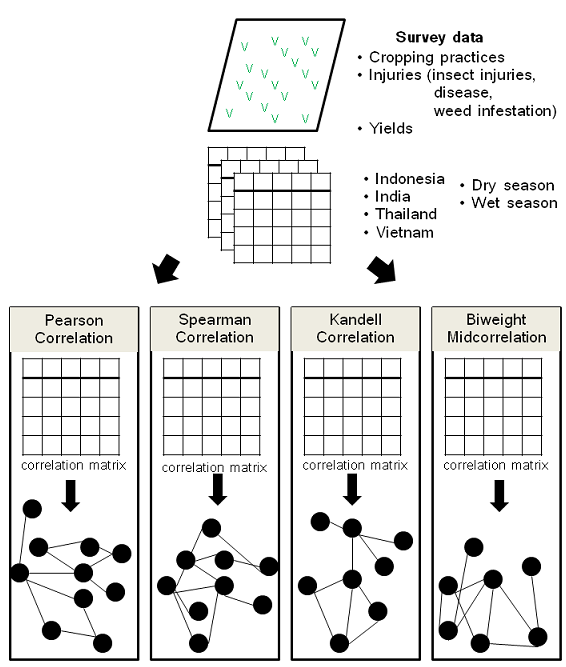
\includegraphics[resolution = 600]{pipeline}
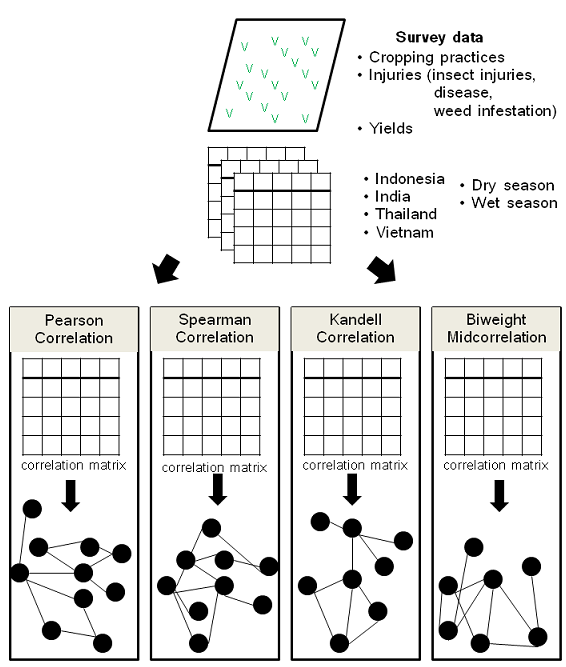
\includegraphics[width = 6in]{pipeline}
% What is FDR correction? A caption should enable a figure to stand on its own.
\caption[Network method for characterizing interactions between injury profiles and cropping practices using correlation measures]{Crop health survey data that were collected include cropping practices, injuries, and yield data. These data were collected from farmers' fields in four countries: Indonesia, India, Thailand, and Vietnam. Correlation matrices will be produced using four individual methods; Pearson, Spearman, Kendall correlation and Biweight midcorrelation. The $p$~values for all coefficients will be adjusted for multiple comparison by false discovery rate (FDR) correction. The correlation coefficients with $p$~values > 0.05 will be removed. The resulting network will be analyzed for structural properties and to infer biological meanings. This will provide the cropping practices and injury profiles network of crop health data.}
\end{figure}
%\end{landscape}

\newpage
\begin{landscape}
\begin{figure}
\centering
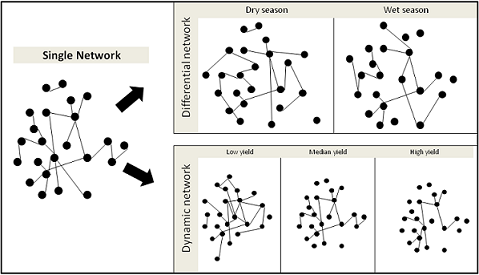
\includegraphics[width=8in]{wholenet}
\caption[Network comparison]{A single network will be created from the whole survey data set. Differential networks will be constructed using different data set, which may be different subgroups of samples from different seasons (\textit{e.g.}, dry season and wet season) or different geographic locations, then differences in connectivity patterns between two networks will be measured. Dynamic networks will be produced from different subgroups of surveys by grouping consecutive yield levels, (\textit{i.e.}, low, median, high yield).}
\end{figure}
\end{landscape}

%================eos================================

%=============================================
% CONCLUSION
%\chapter{Conclusion}
%==============================================
%%===================
% CONCLUSION
%===================
To manage broad range of pests in sustainable way of agriculture, understandings of yield constrains are required priority. Agroecosystems are diverse and complex. Networks are commonly applied to analyze systemic interplay of biological components. Network analysis enables us to the explore the complex biological process and understand holistically. The gene-gene interaction networks, for instance, reveal the gene functions and system. Besides, the emergence properties after network reconstruction give the clues to cluster the components that close related, called hub. Networks are not static when different environment can reprogram the components arrangements and functions. Moreover, networks can allow us the consider the only the elements response the given changes. With versatile applications of network analysis, agroecosystem potentially can be modeled as a network. The new type of information will be proposed from the network analysis. One of the most challenge will be the model evaluation. Because this is the first attempt to applied network into the context of rice agroecosystem. Meeting this goal will require the development the validated methods to integrate heterogeneous data and built different networks on the basis of the particular rice agroecosystem.   




% The \appendix statement indicates the beginning of the appendices.

%----------------------------------------------------------------------
% END MATERIAL
%----------------------------------------------------------------------

% B I B L I O G R A P H Y
% -----------------------

\renewcommand{\bibname}{LITERATURE CITED}
\bibliographystyle{apacite}
\bibliography{reference}
\end{document}
`